\section{Waves}
\footnotetext{Notes based on 3blue1brown/minutephysics \url{https://www.youtube.com/watch?v=MzRCDLre1b4}}

The late 1800s understanding of light (marked by Maxwell's Equations) was that it consists of waves
in the electromagnetic field.

The electromagnetic field comprises an \defn{electric field} and a \defn{magnetic field}. These are
both vector fields: i.e. they consist of a vector-valued quantity at every location $z$ in
3-dimensional space. The field changes over time, so can be written as a vector-valued function
$\va{F}(z, t)$.

{\bf Electric field:} $\va E(z, t)$) Suppose a charged particle is at location $z$. Then there is a
force on the particle dependent on the field value $\va E(z, t)$ and the charge of the particle.

{\bf Magnetic field:} $\va B(z, t)$ Suppose a particle with charge $q$ is moving with velocity
$\va v$ in a magnetic field $\va B(z, t)$. Then there is a force on the particle equal to
$q\va v \times \va B(z, t)$\footnote{$\times$ is a cross product of vector-valued quantities, so
  this means that the direction of the force is perpendicular to both the velocity direction and the
  field direction at that location, and that the magnitude of the force is equal to the product of
  their magnitudes and the charge $q$.}.

Maxwell's equations describe how these two vector fields interact. \footnotetext{In the video, it is
  mentioned that a region of circular flow in one of the fields causes the other field within that
  region to point perpendicular to the plane of the loop.} The one-sentence summary is that in an
electromagnetic wave, the electric and magnetic fields oscillate, perpendicular to each other, and
perpendicular to the direction of propagation.

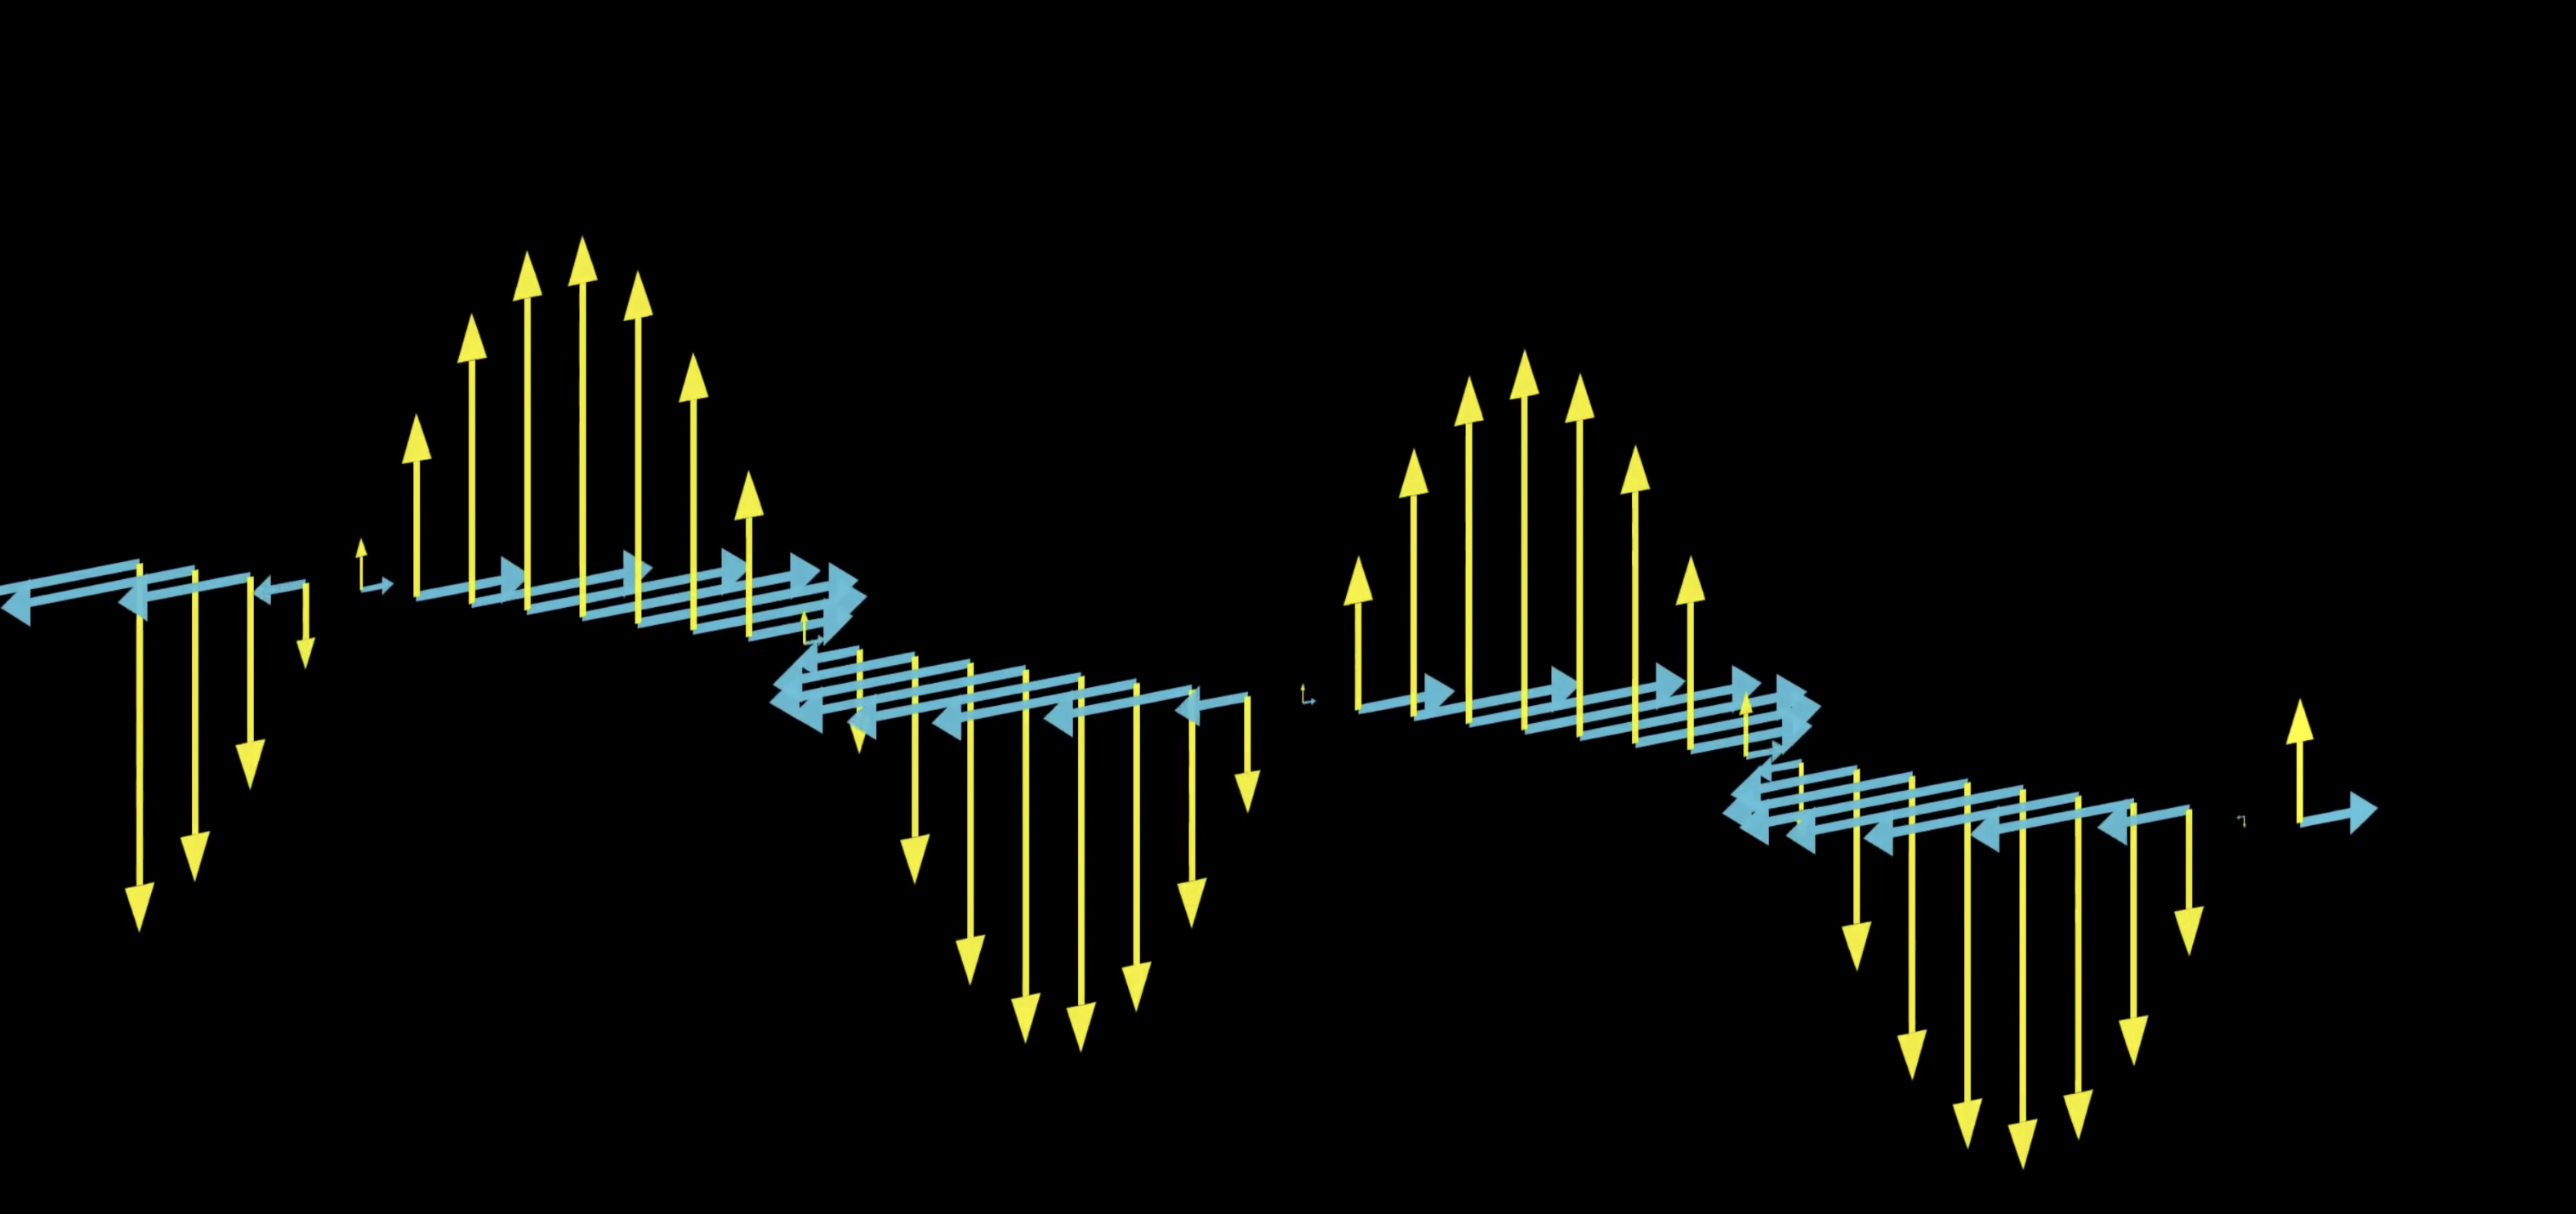
\includegraphics[width=250pt]{img/quantum-waves-1.png}

In the above screenshot, the longitudinal axis of the wave represents space $z$. Time $t$ is
depicted via animation: the vector component of (e.g.) the blue field, at a single spatial location
$z$, grows and shrinks and changes direction over time.

Now we switch perspective to view the wave head-on, focusing on a slice perpendicular to the
direction of propagation of the wave, at a single spatial location.


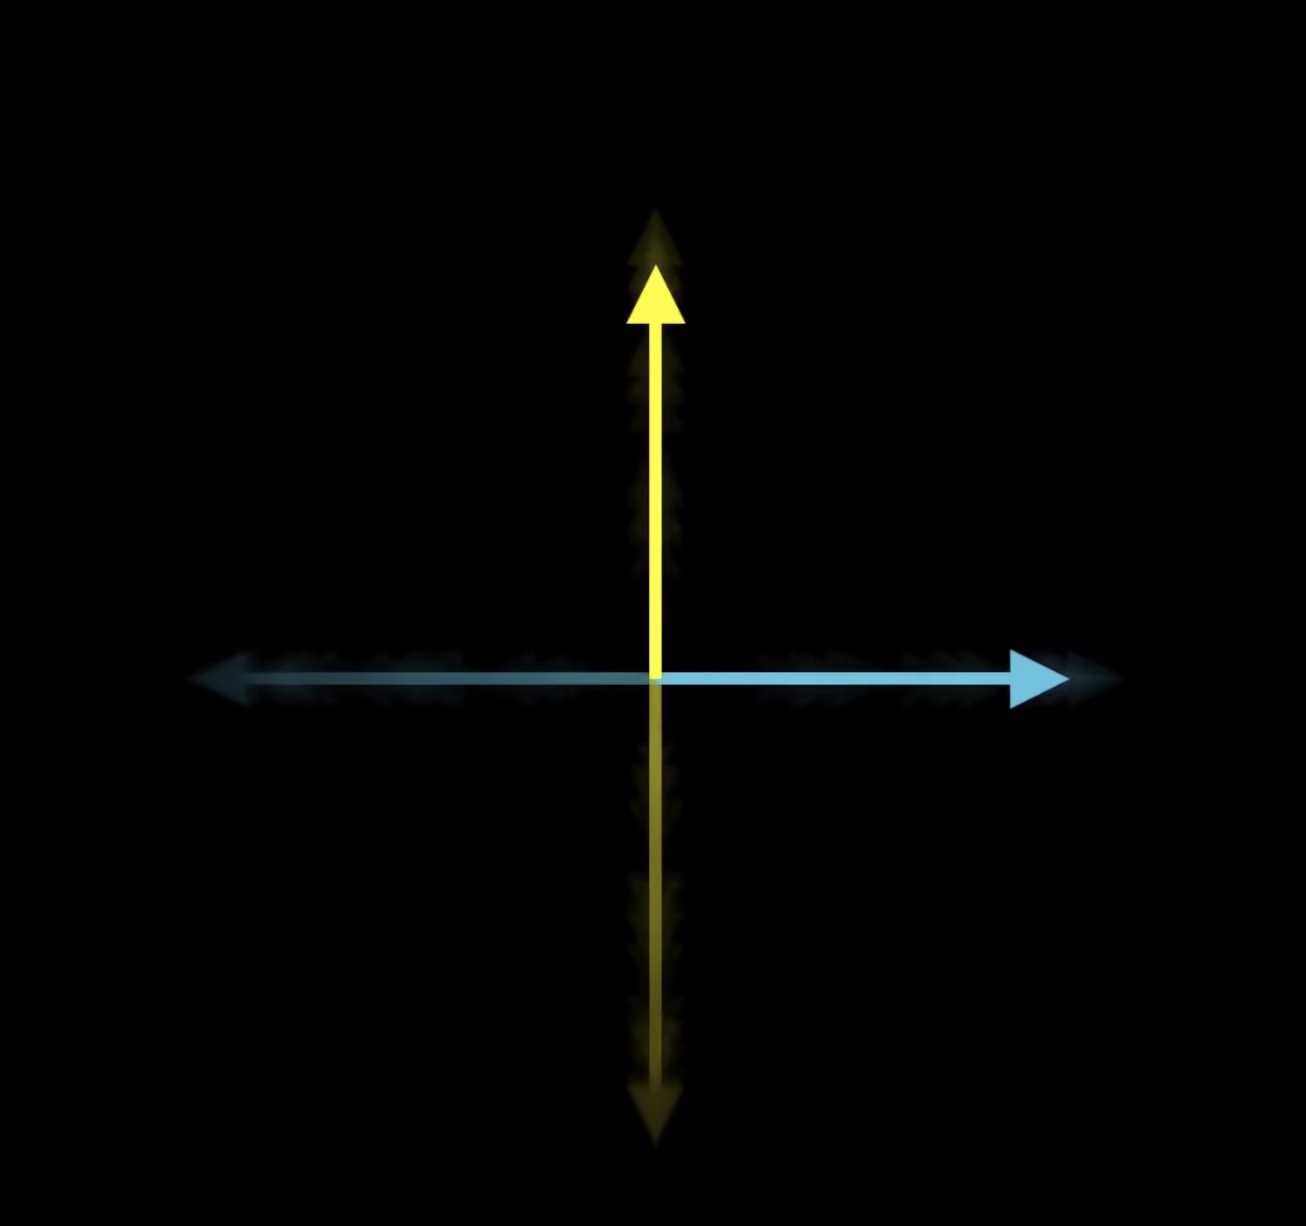
\includegraphics[width=100pt]{img/quantum-waves-2.png}

And we focus on the dynamics of the blue vector component:

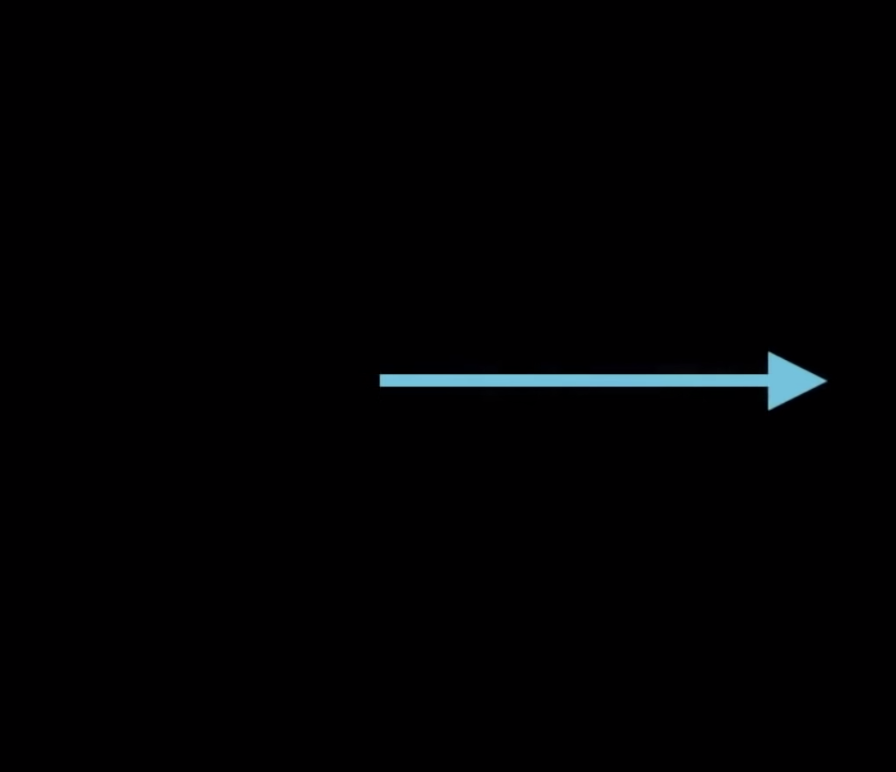
\includegraphics[width=100pt]{img/quantum-waves-3.png}

We use a column vector to represent its position in the left-right ($x$) and up-down ($y$)
directions, as a function of time. Since it is moving horizontally, its up-down value is constant at
zero, and its left-right dynamics can be described by a cosine function of time (with time scaled by
$2\pi$ so that one cosine oscillation is completed in one unit of time):
\begin{align*}
  \va E = \vecMM{\cos(2\pi t)}{0}.
\end{align*}
We include a parameter $f_x$ controlling its frequency of oscillation, and a parameter $A_x$
controlling its amplitude:
\begin{align*}
  \va E = \vecMM{A_x\cos(2\pi f_xt)}{0}.
\end{align*}
And we also include a parameter $\phi_x$ controlling the phase shift of this oscillation, i.e. where
in its cycle it is at time $t=0$:
\begin{align*}
  \va E = \vecMM{A_x\cos(2\pi f_xt + \phi_x)}{0}.
\end{align*}
In quantum mechanics this vector would typically be written instead as a linear combination of basis
vectors (kets):
\begin{align*}
  \va E = A_x \cos(2\pi f_x t + \phi_x) \ket{\rightarrow} + 0\ket{\uparrow}.
\end{align*}

So to recap:
\begin{enumerate}
\item We are considering horizontal oscillation, and vertical oscillation, as two basis vectors in a
  vector space of waves.
\item As usual in a vector space, we form linear combinations of the basis vectors.
\item When forming the linear combination, the weight (scalar) we use to scale a basis vector is a
  quantity with amplitude, frequency and phase shift.
\end{enumerate}

An electromagnetic wave exhibiting pure horizontal (vertical) oscillation is said to be horizontally
(vertically) \defn{polarized}.

A linear combination of the two basis wave types is referred to as a \defn{superposition}.

The wave resulting from the linear combination behaves as follows:
\begin{enumerate}
\item If the coefficients have the same phase shift, then the linear combination wave will be
  polarized along some diagonal direction.
\item If they have different phase shifts then the linear combination wave will ``rotate'', tracing
  out an ellipse (circle if the amplitudes are equal).
\item If their phase shifts differ by $90\deg$ and their amplitudes are equal then the linear
  combination wave traces out a circle and this is said to be \defn{circularly polarized} light.
\end{enumerate}


\newpage
\section{Waves and complex numbers}
\footnotetext{Notes based on \emph{Waves and Complex Numbers} by Mark Van Raamsdonk
  \url{https://www.phas.ubc.ca/~mav/p200/complex.pdf} and \emph{Notes on Complex Numbers in Physics}
  by Paul Cadden-Zimansky
  \url{http://bohr.physics.berkeley.edu/hal/teaching/phys230Sp17/notes/CaddenZimanskysNotesComplexNumbers.pdf}}

A one-dimensional wave is a function of space and time. A single harmonic (pure sinusoidal)
component of a wave might have the form
\begin{align*}
  g(x, t) = A\cos(kx - \omega t + \varphi),
\end{align*}
where
\begin{itemize}
\item $k = 2\pi/\lambda$ is the \defn{wavenumber}, with $\lambda$ the wavelength,
\item $\omega$ is the \defn{angular frequency},
\item $\varphi$ is the \defn{phase}, which determines where the wave is in its cycle at
  $x = 0, t = 0$.
\end{itemize}

So far, nothing involves imaginary numbers.

Now, recall that:
\begin{enumerate}
\item $f(t) = Ae^{it}$ moves around a circle of radius $A$ in the complex plane, completing one
  revolution every $2\pi$ units of time. Its 1D projections trace out a cosine function on the real
  axis, and a sine function on the imaginary axis:
  \begin{align*}
    Ae^{it} = A\cos t + iA\sin t.
  \end{align*}
\item This equation holds when plugging $it$ and $t$ into the respective Taylor series for the
  exponential function and trig functions; its proof would take the Taylor series as definitional.
\end{enumerate}

So we are free to take our real wave function
\begin{align*}
  g(x, t) = A\cos(kx - \omega t + \varphi)
\end{align*}
and consider it to be the real part of a complex exponential function:
\begin{align*}
  \tilde g(x, t) = Ae^{i(kx - \omega t + \varphi)}.
\end{align*}


\newpage
\subsection*{Questions}
\begin{enumerate}
\item Why is it a cosine not a sine? Is that related to the fact that cosine is associated with the
  real component of a complex number??
\item What exactly does ``wave propagation'' mean?
\item In principle, presumably, vectors in the electric and magnetic vector fields can point in any
  direction in 3D space. What are the constraints on this when we are considering a ``wave''?
\item At 6:40, Grant refers to the waves as solutions to Maxwell's Equations. However, we're only
  considering the electric field at this point; wouldn't we have to be considering both electric and
  magnetic for it to be a solution of Maxwell's Equations?
\item So different phase shifts can cause a ``rotating'' wave tracing an elliptical path (circular
  if same amplitude). But what about differences in frequency?
\end{enumerate}

% \newpage
% See \ref{real-and-complex-vector-spaces}
% \section{Adjoint, Unitary matrices, etc}\label{adjoint-and-unitary-matrices}
% The \defn{conjugate transpose} or \defn{adjoint} or \defn{Hermitian conjugate} of a matrix is formed
% by taking the transpose, and then replacing each element with its complex conjugate:
% \begin{align*}
%   U^\dag = \bar{U^T}.
% \end{align*}
% It is also written as $U^*$ or $U^H$.

% A matrix $U$ is \defn{unitary} if $U^\dag U = I$.

% \newpage
% \section{The qubit}
% \footnotetext{Notes based on Michael Nielsen - Quantum Computing for the Very Curious \url{https://quantum.country/qcvc}}

% The state of a qubit is a unit vector in a two-dimensional complex vector space. The basis vectors
% are written $\ket{0}$ and $\ket{1}$, so a qubit is
% \begin{align*}
%   \alpha\ket{0} + \beta\ket{1}
% \end{align*}
% where $\alpha, \beta \in \C$ with $|\alpha|^2 + |\beta|^2 = 1$.

% What does the normalization constraint $|\alpha|^2 + |\beta|^2 = 1$ mean geometrically? If
% $\alpha = 0$ then $\beta$ lies on the unit circle, and vice versa.

% How can we visualize the possible values of a qubit?

% Perhaps like this? This diagram illustrates that we pick two complex numbers, $\alpha$ and $\beta$,
% and that they satisfy $|\alpha|^2 + |\beta^2| = 1$.\\
% 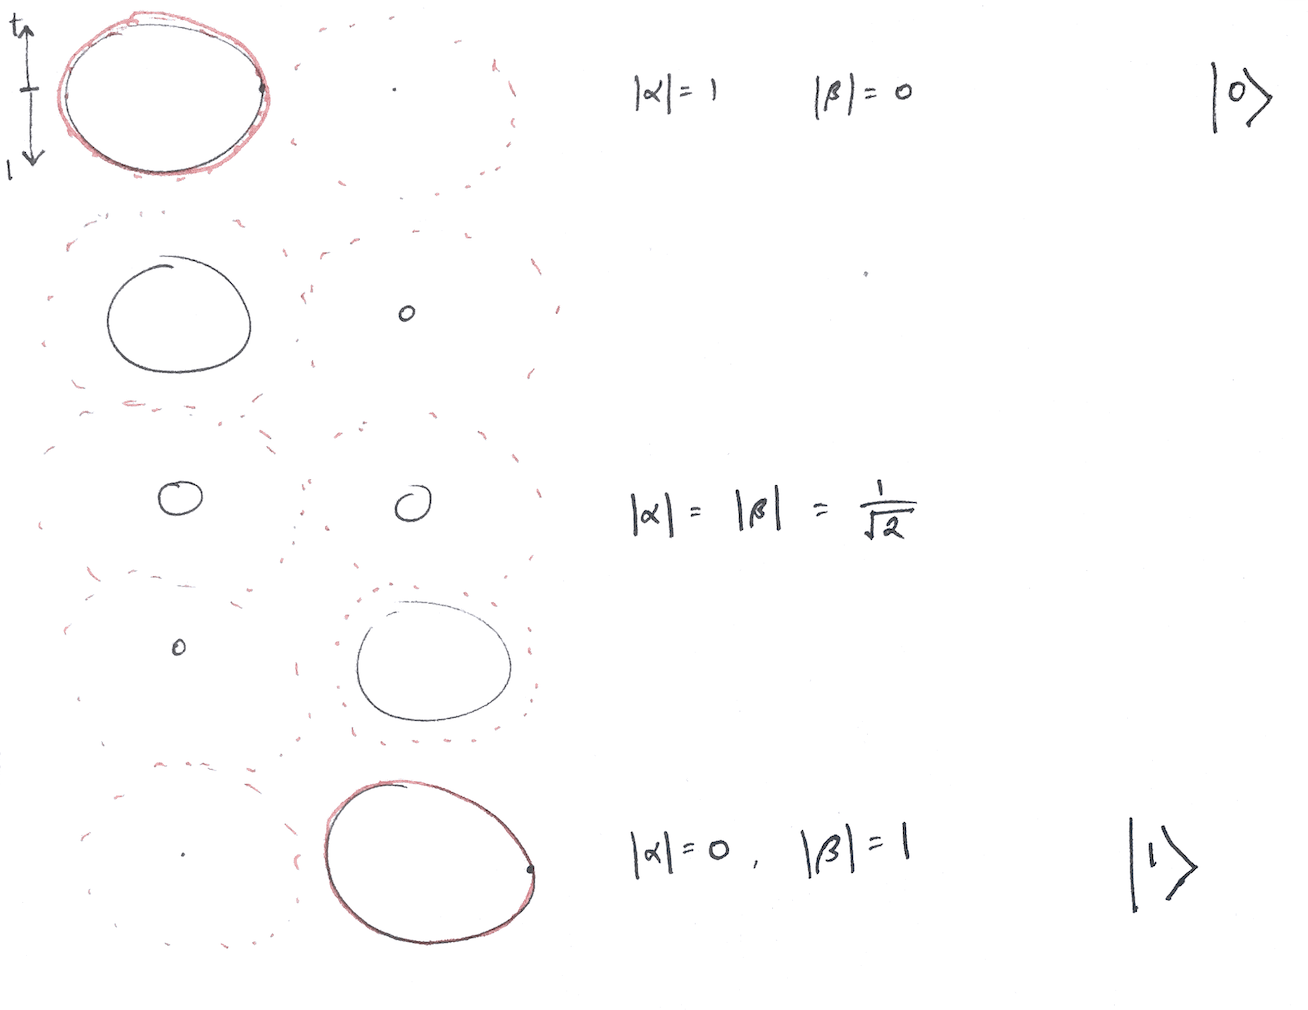
\includegraphics[width=200pt]{img/quantum-qubit-2.png}

% Or like this? Visualize $(|\alpha|, |\beta|)$ as a point on the unit circle and place a clockface at
% that point with two hands, representing the argument
% of $\alpha$ and $\beta$.\\
% 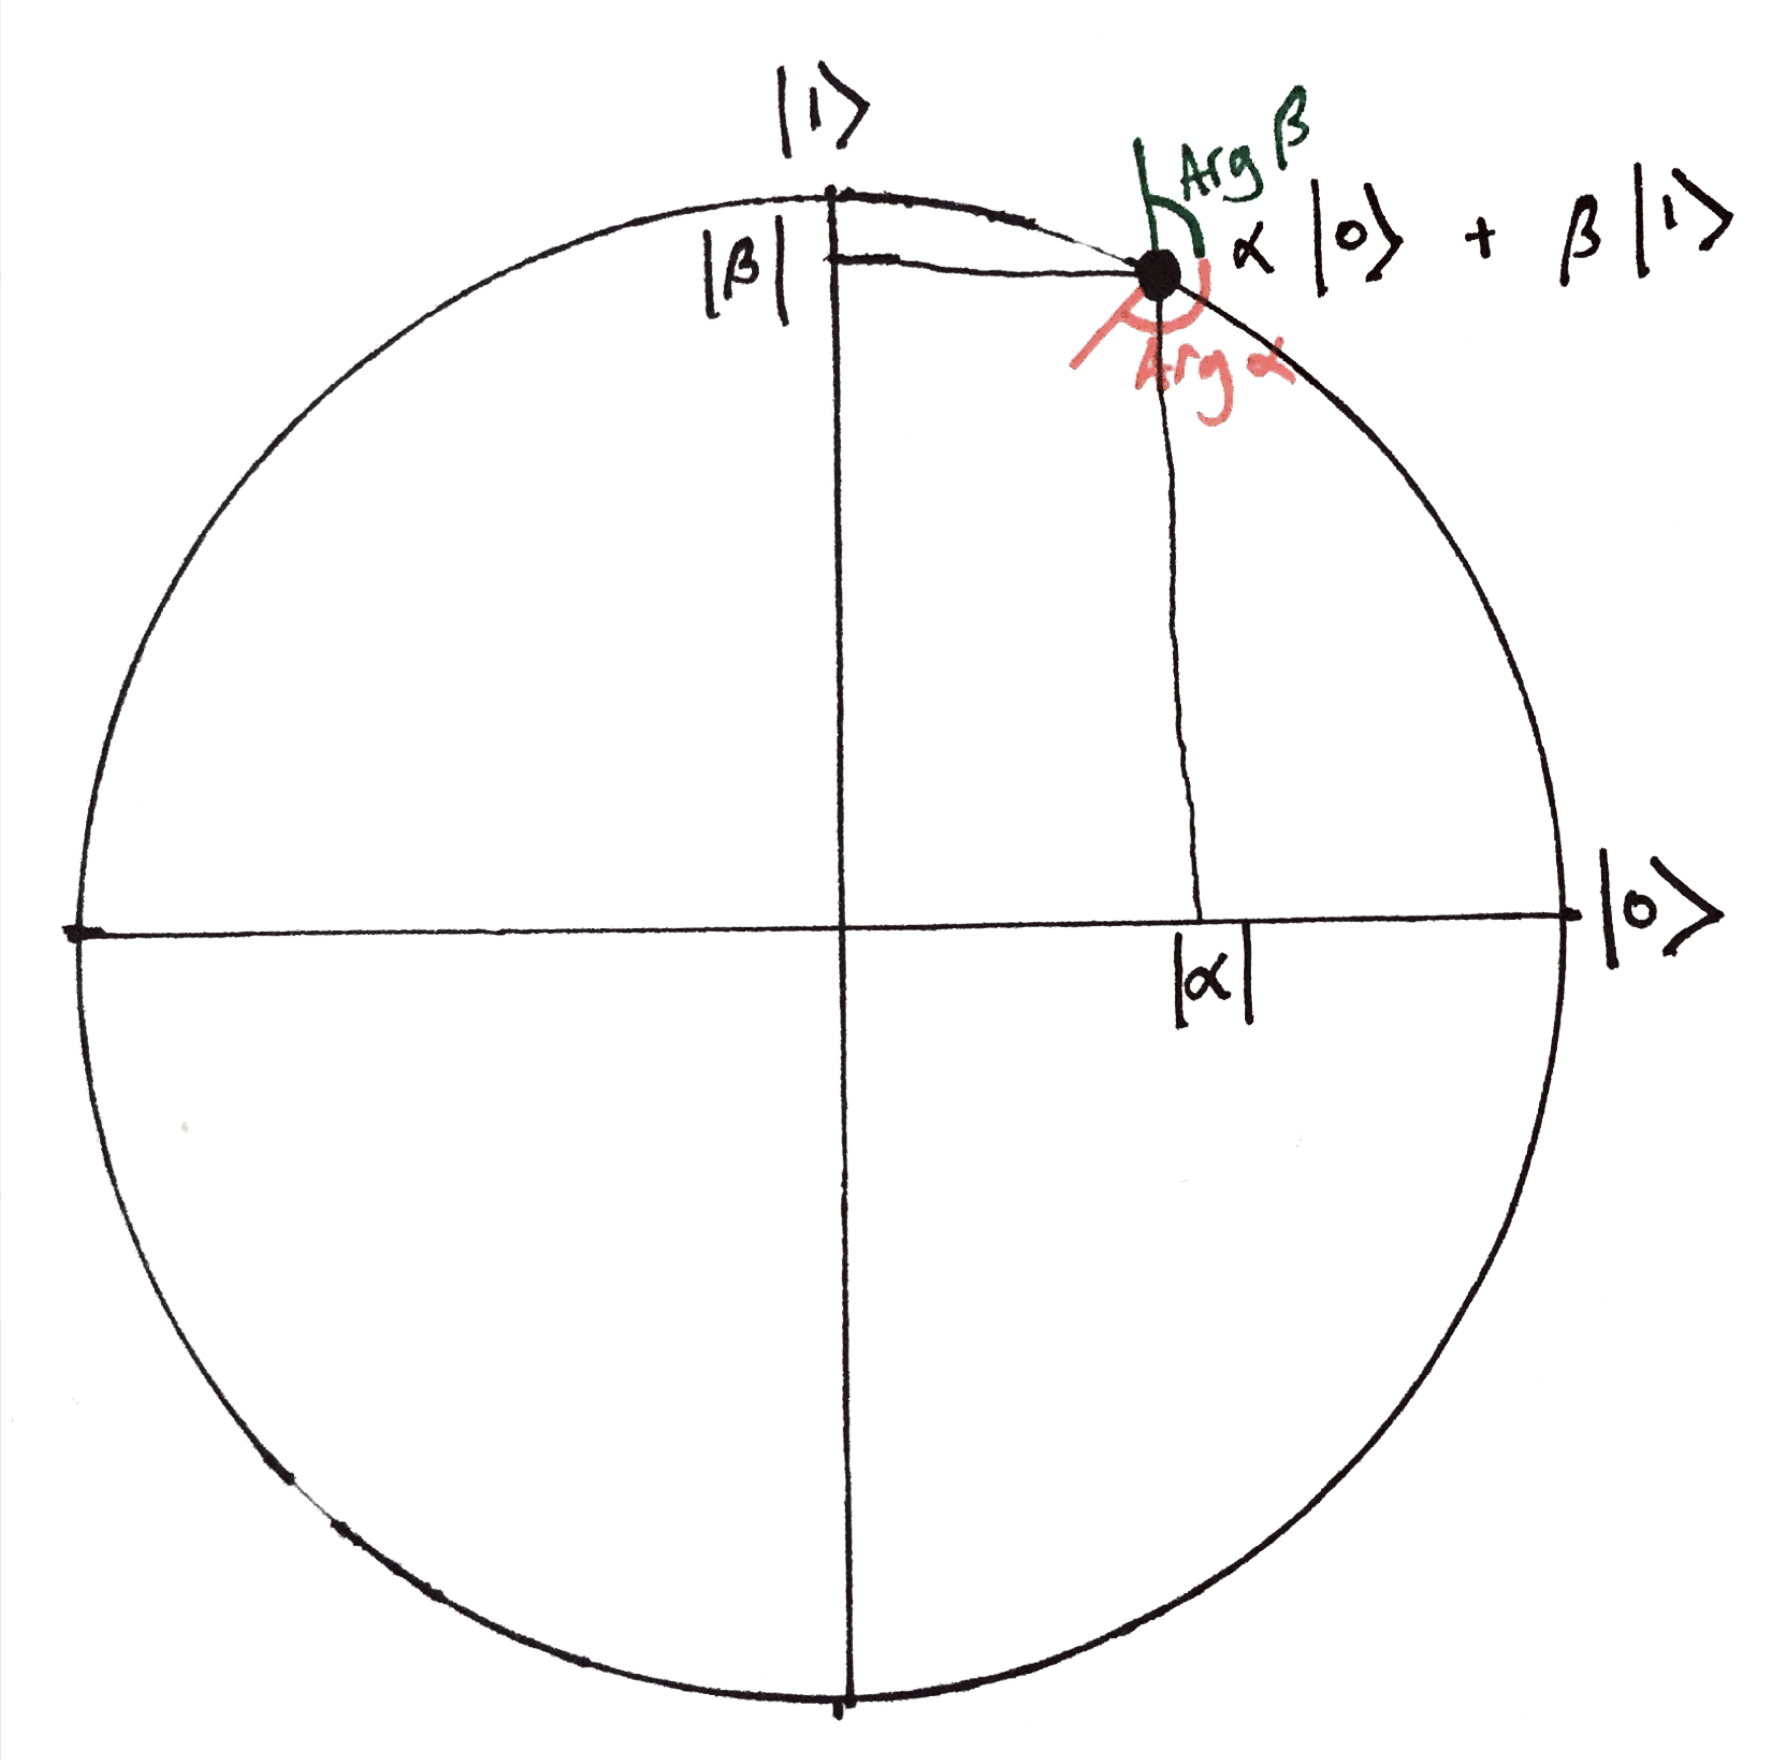
\includegraphics[width=200pt]{img/quantum-qubit.png}


% \newpage


% \newpage
% \section{Quantum logic gates}

% These are linear operators that act on a qubit state to produce a new qubit state. Therefore they
% are $2 \times 2$ complex matrices. Since they unitary
% \begin{enumerate}
% \item {\bf Not}
%   \begin{align*}
%     X = \matMMxNN{0}{1}
%     {1}{0}
%   \end{align*}
% \item {\bf Hadamard}
%   \begin{align*}
%     H = \frac{1}{\sqrt{2}}\matMMxNN{1}{1}
%     {1}{-1}
%   \end{align*}
% \item {\bf $Y$}
%   \begin{align*}
%     Y = \matMMxNN{0}{-i}
%                  {i}{0}
%   \end{align*}
% \item {\bf $Z$}
%   \begin{align*}
%     Z = \matMMxNN{1}{0}
%                  {0}{-1}
%   \end{align*}
% \end{enumerate}

% The not gate essentially swaps the two dimensions: the coefficient of $\ket{0}$ becomes the
% coefficient of $\ket{1}$ and vice versa. So e.g.
% \begin{align*}
%   X\ket{0} &= \ket{1}\\
%   X\ket{1} &= \ket{0},
% \end{align*}
% and by linearity
% \begin{align*}
%   X \(\alpha \ket{0} + \beta \ket{1}\) = \beta \ket{0} + \alpha \ket{1}
% \end{align*}

% Since they are real and symmetric, we have $X^\dag = X$ and $H^\dag = H$. And since
% \begin{align*}
%   X^2 &= I\\
%   H^2 &= \frac{1}{2}\matMMxNN{2}{0}
%         {0}{2} = I,
% \end{align*}\
% we have that $X$ and $H$ are unitary.


% % \begin{align*}
% %   H \ket{0} &= \frac{\ket{0}}{\sqrt{2}} + \frac{\ket{1}}{\sqrt{2}}\\
% %   H \ket{1} &= \frac{\ket{0}}{\sqrt{2}} - \frac{\ket{1}}{\sqrt{2}}
% % \end{align*}
